% Options for packages loaded elsewhere
\PassOptionsToPackage{unicode}{hyperref}
\PassOptionsToPackage{hyphens}{url}
%
\documentclass[
]{article}
\usepackage{lmodern}
\usepackage{amssymb,amsmath}
\usepackage{ifxetex,ifluatex}
\ifnum 0\ifxetex 1\fi\ifluatex 1\fi=0 % if pdftex
  \usepackage[T1]{fontenc}
  \usepackage[utf8]{inputenc}
  \usepackage{textcomp} % provide euro and other symbols
\else % if luatex or xetex
  \usepackage{unicode-math}
  \defaultfontfeatures{Scale=MatchLowercase}
  \defaultfontfeatures[\rmfamily]{Ligatures=TeX,Scale=1}
\fi
% Use upquote if available, for straight quotes in verbatim environments
\IfFileExists{upquote.sty}{\usepackage{upquote}}{}
\IfFileExists{microtype.sty}{% use microtype if available
  \usepackage[]{microtype}
  \UseMicrotypeSet[protrusion]{basicmath} % disable protrusion for tt fonts
}{}
\makeatletter
\@ifundefined{KOMAClassName}{% if non-KOMA class
  \IfFileExists{parskip.sty}{%
    \usepackage{parskip}
  }{% else
    \setlength{\parindent}{0pt}
    \setlength{\parskip}{6pt plus 2pt minus 1pt}}
}{% if KOMA class
  \KOMAoptions{parskip=half}}
\makeatother
\usepackage{xcolor}
\IfFileExists{xurl.sty}{\usepackage{xurl}}{} % add URL line breaks if available
\IfFileExists{bookmark.sty}{\usepackage{bookmark}}{\usepackage{hyperref}}
\hypersetup{
  pdftitle={gtsummary},
  pdfauthor={Daniel D. Sjoberg, Karissa Whiting, Margaret Hannum, Emily C. Zabor, Michael Curry},
  hidelinks,
  pdfcreator={LaTeX via pandoc}}
\urlstyle{same} % disable monospaced font for URLs
\usepackage[margin=1in]{geometry}
\usepackage{color}
\usepackage{fancyvrb}
\newcommand{\VerbBar}{|}
\newcommand{\VERB}{\Verb[commandchars=\\\{\}]}
\DefineVerbatimEnvironment{Highlighting}{Verbatim}{commandchars=\\\{\}}
% Add ',fontsize=\small' for more characters per line
\usepackage{framed}
\definecolor{shadecolor}{RGB}{248,248,248}
\newenvironment{Shaded}{\begin{snugshade}}{\end{snugshade}}
\newcommand{\AlertTok}[1]{\textcolor[rgb]{0.94,0.16,0.16}{#1}}
\newcommand{\AnnotationTok}[1]{\textcolor[rgb]{0.56,0.35,0.01}{\textbf{\textit{#1}}}}
\newcommand{\AttributeTok}[1]{\textcolor[rgb]{0.77,0.63,0.00}{#1}}
\newcommand{\BaseNTok}[1]{\textcolor[rgb]{0.00,0.00,0.81}{#1}}
\newcommand{\BuiltInTok}[1]{#1}
\newcommand{\CharTok}[1]{\textcolor[rgb]{0.31,0.60,0.02}{#1}}
\newcommand{\CommentTok}[1]{\textcolor[rgb]{0.56,0.35,0.01}{\textit{#1}}}
\newcommand{\CommentVarTok}[1]{\textcolor[rgb]{0.56,0.35,0.01}{\textbf{\textit{#1}}}}
\newcommand{\ConstantTok}[1]{\textcolor[rgb]{0.00,0.00,0.00}{#1}}
\newcommand{\ControlFlowTok}[1]{\textcolor[rgb]{0.13,0.29,0.53}{\textbf{#1}}}
\newcommand{\DataTypeTok}[1]{\textcolor[rgb]{0.13,0.29,0.53}{#1}}
\newcommand{\DecValTok}[1]{\textcolor[rgb]{0.00,0.00,0.81}{#1}}
\newcommand{\DocumentationTok}[1]{\textcolor[rgb]{0.56,0.35,0.01}{\textbf{\textit{#1}}}}
\newcommand{\ErrorTok}[1]{\textcolor[rgb]{0.64,0.00,0.00}{\textbf{#1}}}
\newcommand{\ExtensionTok}[1]{#1}
\newcommand{\FloatTok}[1]{\textcolor[rgb]{0.00,0.00,0.81}{#1}}
\newcommand{\FunctionTok}[1]{\textcolor[rgb]{0.00,0.00,0.00}{#1}}
\newcommand{\ImportTok}[1]{#1}
\newcommand{\InformationTok}[1]{\textcolor[rgb]{0.56,0.35,0.01}{\textbf{\textit{#1}}}}
\newcommand{\KeywordTok}[1]{\textcolor[rgb]{0.13,0.29,0.53}{\textbf{#1}}}
\newcommand{\NormalTok}[1]{#1}
\newcommand{\OperatorTok}[1]{\textcolor[rgb]{0.81,0.36,0.00}{\textbf{#1}}}
\newcommand{\OtherTok}[1]{\textcolor[rgb]{0.56,0.35,0.01}{#1}}
\newcommand{\PreprocessorTok}[1]{\textcolor[rgb]{0.56,0.35,0.01}{\textit{#1}}}
\newcommand{\RegionMarkerTok}[1]{#1}
\newcommand{\SpecialCharTok}[1]{\textcolor[rgb]{0.00,0.00,0.00}{#1}}
\newcommand{\SpecialStringTok}[1]{\textcolor[rgb]{0.31,0.60,0.02}{#1}}
\newcommand{\StringTok}[1]{\textcolor[rgb]{0.31,0.60,0.02}{#1}}
\newcommand{\VariableTok}[1]{\textcolor[rgb]{0.00,0.00,0.00}{#1}}
\newcommand{\VerbatimStringTok}[1]{\textcolor[rgb]{0.31,0.60,0.02}{#1}}
\newcommand{\WarningTok}[1]{\textcolor[rgb]{0.56,0.35,0.01}{\textbf{\textit{#1}}}}
\usepackage{graphicx,grffile}
\makeatletter
\def\maxwidth{\ifdim\Gin@nat@width>\linewidth\linewidth\else\Gin@nat@width\fi}
\def\maxheight{\ifdim\Gin@nat@height>\textheight\textheight\else\Gin@nat@height\fi}
\makeatother
% Scale images if necessary, so that they will not overflow the page
% margins by default, and it is still possible to overwrite the defaults
% using explicit options in \includegraphics[width, height, ...]{}
\setkeys{Gin}{width=\maxwidth,height=\maxheight,keepaspectratio}
% Set default figure placement to htbp
\makeatletter
\def\fps@figure{htbp}
\makeatother
\setlength{\emergencystretch}{3em} % prevent overfull lines
\providecommand{\tightlist}{%
  \setlength{\itemsep}{0pt}\setlength{\parskip}{0pt}}
\setcounter{secnumdepth}{-\maxdimen} % remove section numbering

\title{gtsummary}
\author{Daniel D. Sjoberg, Karissa Whiting, Margaret Hannum, Emily C. Zabor,
Michael Curry}
\date{}

\begin{document}
\maketitle

\hypertarget{introduction}{%
\section{Introduction}\label{introduction}}

\hypertarget{data-summaries}{%
\section{Data Summaries}\label{data-summaries}}

\% latex comment ?

\hypertarget{tbl_summary}{%
\subsection{\texorpdfstring{\texttt{tbl\_summary()}}{tbl\_summary()}}\label{tbl_summary}}

\begin{Shaded}
\begin{Highlighting}[]
\NormalTok{tbl_summary_}\DecValTok{1}\NormalTok{ <-}
\StringTok{  }\NormalTok{trial }\OperatorTok
\StringTok{  }\KeywordTok{select}\NormalTok{(age, grade, response, trt) }\OperatorTok
\StringTok{  }\KeywordTok{tbl_summary}\NormalTok{(}\DataTypeTok{by =}\NormalTok{ trt)}
\end{Highlighting}
\end{Shaded}

\begin{Shaded}
\begin{Highlighting}[]
\NormalTok{tbl_summary_}\DecValTok{2}\NormalTok{ <-}
\StringTok{  }\NormalTok{trial }\OperatorTok
\StringTok{  }\KeywordTok{select}\NormalTok{(age, grade, response, trt) }\OperatorTok
\StringTok{  }\KeywordTok{tbl_summary}\NormalTok{(}
    \DataTypeTok{by =}\NormalTok{ trt,}
    \DataTypeTok{type =} \KeywordTok{all_continuous}\NormalTok{() }\OperatorTok{~}\StringTok{ "continuous2"}\NormalTok{,}
    \DataTypeTok{label =}\NormalTok{ age }\OperatorTok{~}\StringTok{ "Patient Age"}\NormalTok{,}
    \DataTypeTok{statistic =} \KeywordTok{list}\NormalTok{(}\KeywordTok{all_continuous}\NormalTok{() }\OperatorTok{~}\StringTok{ }\KeywordTok{c}\NormalTok{(}\StringTok{"\{N_nonmiss\}"}\NormalTok{, }
                                          \StringTok{"\{mean\} (\{sd\})"}\NormalTok{, }
                                          \StringTok{"\{median\} (\{p25\}, \{p75\})"}\NormalTok{, }
                                          \StringTok{"\{min\}, \{max\}"}\NormalTok{),}
                     \KeywordTok{all_categorical}\NormalTok{() }\OperatorTok{~}\StringTok{ "\{n\} / \{N\} (\{p\}%)"}\NormalTok{),}
    \DataTypeTok{digits =} \KeywordTok{all_categorical}\NormalTok{() }\OperatorTok{~}\StringTok{ }\KeywordTok{c}\NormalTok{(}\DecValTok{0}\NormalTok{, }\DecValTok{0}\NormalTok{, }\DecValTok{1}\NormalTok{),}
    \DataTypeTok{missing =} \StringTok{"no"}
\NormalTok{  )}
\end{Highlighting}
\end{Shaded}

\begin{Shaded}
\begin{Highlighting}[]
\NormalTok{tbl_summary_}\DecValTok{3}\NormalTok{ <-}
\StringTok{  }\NormalTok{trial }\OperatorTok
\StringTok{  }\KeywordTok{select}\NormalTok{(age, grade, response, trt) }\OperatorTok
\StringTok{  }\KeywordTok{tbl_summary}\NormalTok{(}\DataTypeTok{by =}\NormalTok{ trt, }\DataTypeTok{missing =} \StringTok{"no"}\NormalTok{) }\OperatorTok
\StringTok{  }\KeywordTok{add_p}\NormalTok{(}\DataTypeTok{test =} \KeywordTok{all_continuous}\NormalTok{() }\OperatorTok{~}\StringTok{ "t.test"}\NormalTok{,}
        \DataTypeTok{pvalue_fun =} \OperatorTok{~}\KeywordTok{style_pvalue}\NormalTok{(., }\DataTypeTok{digits =} \DecValTok{2}\NormalTok{)) }\OperatorTok
\StringTok{  }\KeywordTok{add_n}\NormalTok{()}
\end{Highlighting}
\end{Shaded}

\begin{figure}[h!]
  \caption{Simple `tbl\_summary()` example}
  \label{fig:summary_basic}
  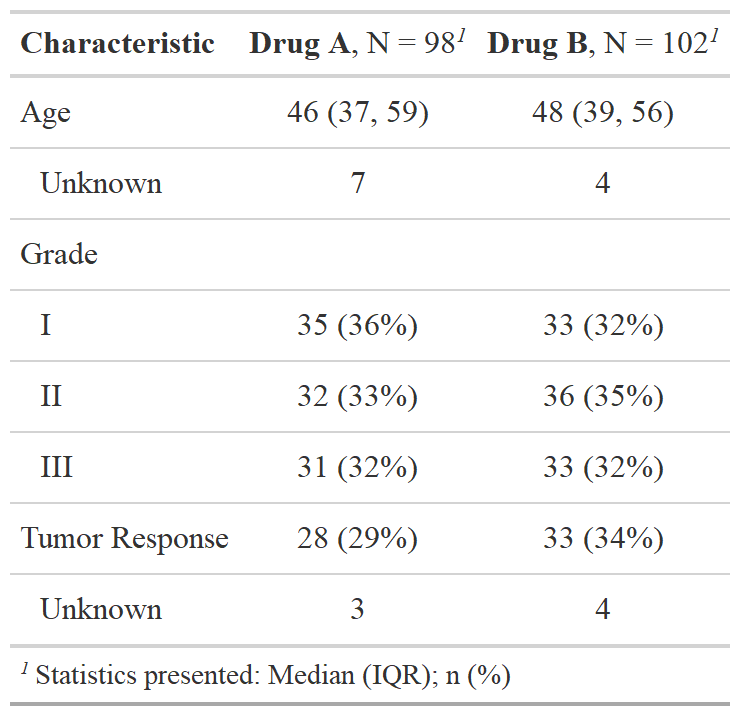
\includegraphics[height=5cm]{summary_basic.png}
  \centering
\end{figure}

\hypertarget{tbl_svysummary}{%
\subsection{\texorpdfstring{\texttt{tbl\_svysummary()}}{tbl\_svysummary()}}\label{tbl_svysummary}}

\hypertarget{tbl_cross}{%
\subsection{\texorpdfstring{\texttt{tbl\_cross()}}{tbl\_cross()}}\label{tbl_cross}}

\hypertarget{tbl_survfit}{%
\subsection{\texorpdfstring{\texttt{tbl\_survfit()}}{tbl\_survfit()}}\label{tbl_survfit}}

\hypertarget{customization}{%
\subsection{Customization}\label{customization}}

\hypertarget{model-summaries}{%
\section{Model Summaries}\label{model-summaries}}

\hypertarget{tbl_regression}{%
\subsection{\texorpdfstring{\texttt{tbl\_regression()}}{tbl\_regression()}}\label{tbl_regression}}

\hypertarget{tbl_uvregression}{%
\subsection{\texorpdfstring{\texttt{tbl\_uvregression()}}{tbl\_uvregression()}}\label{tbl_uvregression}}

\hypertarget{merging-and-stacking}{%
\section{Merging and Stacking}\label{merging-and-stacking}}

\hypertarget{inline-reporting}{%
\section{Inline Reporting}\label{inline-reporting}}

To report the result for \texttt{age}, use the following commands
inline.

\begin{quote}
\texttt{\textasciigrave{}r\ inline\_text(tbl\_uvregression\_1,\ variable\ =\ age)\textasciigrave{}}
\end{quote}

Here's how the line will appear in your report.

\begin{quote}
1.02 (95\% CI 1.00, 1.04; p=0.091)
\end{quote}

\hypertarget{themes}{%
\section{Themes}\label{themes}}

\begin{Shaded}
\begin{Highlighting}[]
\KeywordTok{theme_gtsummary_journal}\NormalTok{(}\StringTok{"nejm"}\NormalTok{)}

\NormalTok{tbl_nejm <-}
\StringTok{  }\KeywordTok{glm}\NormalTok{(response }\OperatorTok{~}\StringTok{ }\NormalTok{age }\OperatorTok{+}\StringTok{ }\NormalTok{grade, trial, }\DataTypeTok{family =}\NormalTok{ binomial) }\OperatorTok
\StringTok{  }\KeywordTok{tbl_regression}\NormalTok{(}\DataTypeTok{exponentiate =} \OtherTok{TRUE}\NormalTok{)}
\end{Highlighting}
\end{Shaded}

\hypertarget{print-engines}{%
\section{Print Engines}\label{print-engines}}

\end{document}
